\normalfont\documentclass[letterpaper,11pt]{article}
\usepackage{amsmath, amsfonts,amssymb,latexsym}
\usepackage{fullpage}
\usepackage{parskip}
\usepackage{graphicx}

\begin{document}

\newcommand{\header}{
	\noindent \fbox{
	\begin{minipage}{6.4in}
  	\medskip
  	\textbf{ACM algorithm practice} \hfill \textbf{Fall 2015} \\[1mm]
  	\begin{center}
    	{\Large Week 1 Problems} \\[3mm]
  	\end{center}
	\today \hfill \itshape{Timothy Johnson}
	\medskip
	\end{minipage}}
}

\bigskip
%\header

\section*{Problem 1: Run for beer}
People in BubbleLand like to drink beer. Little do they know, beer here is so good and strong that every time they drink it their speed is 10 times slower than before they drank it.

Birko lives in the city Beergrade, but wants to go to the city Beerburg. You are given a road map of BubbleLand and you need to find the fastest way for him. When he starts his journey in Beergrade his speed is 1. When he comes to a new city he always tries a glass of local beer, which divides his speed by 10.

The question here is what the minimal time is for him to reach Beerburg. If there are several paths with the same minimal time, pick the one that has fewest roads on it. If there is still more than one path, pick any.

It is guaranteed that there will be at least one path from Beergrade to Beerburg.

\textbf{Input} \newline
The first line of input contains an integer $N$, the number of cities in Bubbleland, and an integer $M$, the number of roads in this country. Cities are enumerated from 0 to $N - 1$, with city 0 being Beergrade, and city $N - 1$ being Beerburg. Each of the following $M$ lines contains three integers $a, b, len$, where $a \neq b$. These numbers indicate that there is a bidirectional road between cities $a$ and $b$ with length $len$.

The problem sizes are: $2 \leq N \leq 10^5$, $1 \leq M \leq 10^5$, $0 \leq len \leq 9$. There is at most one road joining any two cities.

\textbf{Output} \newline
The first line of output should contain the minimal time neeed to go from Beergrade to Beerburg. The second line should contain the number of cities on this shortest path. The final line should contain the numbers of the cities on this path in the order they are visited, separated by spaces.

\textbf{Examples}
\begin{itemize}
\item \textbf{Input} \newline
8 10 \newline
0 1 1 \newline
1 2 5 \newline
2 7 6 \newline
0 3 2 \newline
3 7 3 \newline
0 4 0 \newline
4 5 0 \newline
5 7 2 \newline
0 6 0 \newline
6 7 7

\textbf{Output} \newline
32 \newline
3 \newline
0 3 7
\end{itemize}

\subsection*{Solution}
(This one hasn't been implemented yet, sorry. But the implementation step isn't that hard.) \newline
Since we need to find a shortest path, our first instinct is probably to use Dijkstra's algorithm. However, if we start from the beginning and search to the end, we might not find the optimal solution. This is because if we are given a path from the start, the cost to reach the next node depends both on the length of the path to our current node and the number of edges in that path.

However, if we search from the end, then suppose we have a path from $x$ to the end of length $x$. If we want to add another edge at the beginning of the path with length $y$, we know that the total cost of the new path will be $10x + y$. We need the factor of 10 because traversing the first link and drinking the first beer decreases our initial speed by a factor of 10.

Since this is monotonic in $x$ (i.e., it increases whenever $x$ increases), we know that we will visit our nodes in the order of their distance from the end. Therefore, we can run Dijkstra's algorithm from the end, and stop when we reach the beginning. The only catch is that, as stated above, the cost of a new node in our queue will be $10x + y$ instead of $x + y$.

\newpage


\section*{Problem 2: 250250}
(Taken from: https://projecteuler.net/problem=250) \newline

Find the number of non-empty subsets of $\{1^1, 2^2, 3^3, \ldots, 250250^{250250}\}$, the sum of whose elements is divisible by 250. Enter the rightmost 16 digits as your answer.


\subsection*{Solution}
This problem has two main steps. The first is modular exponentiation, and the second is dynamic programming.

First, we note that we only care about the remainder when we divide each of the values in our list by 250. So simplify each value to $i^i (\mod 250)$. This can be computed efficiently using modular exponentiation.

The second step is to find how many subsets of our list sum to each of the 250 possible values modulo 250. We add the values from our list one at a time. We can use any of our previous subsets without our new value, or we can add our new value as a singleton set, or we can add our new value to any of the previous subsets.

For example, suppose that our new value is a 5. In addition to all of the previous subsets, we can increment the number of subsets with a total sum of 5. Then we can take any previous subset with total sum $i$ and add our new value to get a new subset with total sum $(i + 5) \mod 250$.

This will take one scan of our list of 250 possible sums for each of the 250250 elements in our list of possible values to choose, which will be almost instantaneous for a reasonable computer.

\section*{Problem 3: Crack-Free Walls}
(Taken from: https://projecteuler.net/problem=215) \newline
Consider the problem of building a wall out of $2 \times 1$ and $3 \times 1$ bricks (horizontal and vertical dimensions) such that, for extra strength, the gaps between horizontally-adjacent bricks never line up in consecutive layers, i.e., never form a running crack.

For example, the following $9 \times 3$ wall is not acceptable due to the running crack shown in red:

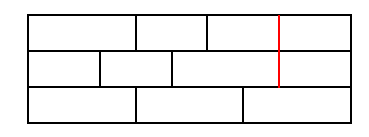
\includegraphics{PE215_fig.png}

There are eight ways of forming a crack-free $9 \times 3$ wall, written $W(9,3) = 8$.

Calculate $W(32,10)$.

Note: Project Euler problems have no enforced time limit, but there is always a solution that takes well under a minute in a reasonably fast language on a standard computer.

\subsection*{Solution}
Our first step is to find all of the possible rows of length 32. It turns out that there are not too many. For example, when we have seven $2 \times 1$ blocks and six $3 \times 1$ blocks, then the total number of ways to arrange them is $\binom{13}{6} = 1716$. The other possible combinations have smaller values, giving a total of 3329 possible rows.

We will now construct a graph in which the nodes are the distinct rows of blocks, and there is an edge between two nodes if those rows can legally be stacked on top of one another. We do a brute force comparison for all of the possible pairs of rows to find which edges to include.

Finally, we add a start node with a directed edge to each of the possible row nodes, and an end node with a directed edge from each of the possible row nodes. Now a path of length $k + 1$ through our graph represents a crack-free wall of height $k$. So we want to count the number of possible paths through our graph from the start to end node with length 11.

The easiest way to do this is to exponentiate the adjacency matrix for our graph. If we let $M$ be our adjacency matrix, then $M^{11}[i][j]$ will represent the number of paths from $i$ to $j$ of length 11. This is the most expensive step, taking time $10n^3$ using a naive algorithm. But this is still doable in several seconds. (My code uses the built-in numpy algorithm for matrix powers, which likely is somewhat faster than the naive solution.)

\end{document}